\section{Semantic Tableaux for first-order logic}

\begin{center}
\textbf{Quantifier rules for Semantic Tableaux}
\end{center}
\begin{tabular}{l c l c}
($ \forall $ T) &  \parbox{5cm}{\centering$ \forall x A(x) : $ T
\newline
$ \downarrow $
\newline
$ A(t/x) : $ T
\newline
for any term \textit{t} occurring on this branch and free for \textit{x} in \textit{A}} & ($ \exists $ T)* & \parbox{5cm}{\centering$ \exists x A(x) : $ T
\newline
$ \downarrow $
\newline
$ A(c/x) : $ T
\newline
for a \textit{new} constant symbol \textit{c} not yet occurring on this branch}  \\[1.5cm]

($ \exists $ F) & \parbox{5cm}{\centering$ \exists x A(x) : $ F
\newline
$ \downarrow $
\newline
$ A(t/x) : $ F
\newline
for any term \textit{t} occurring on this branch and free for \textit{x} in \textit{A}} & ($ \forall $ F)*  & \parbox{5cm}{\centering$ \forall x A(x) : $ F
\newline
$ \downarrow $
\newline
$ A(c/x) : $ F
\newline
for a \textit{new} constant symbol \textit{c} not yet occurring on this branch}  \\
\end{tabular}

(*) \textit{This rule may only be applied once for the given formula on each branch}

Here are some examples of a semantic tableaux with first-order logic \cite[p. 46]{LecPartII}.

\begin{figure}[H]
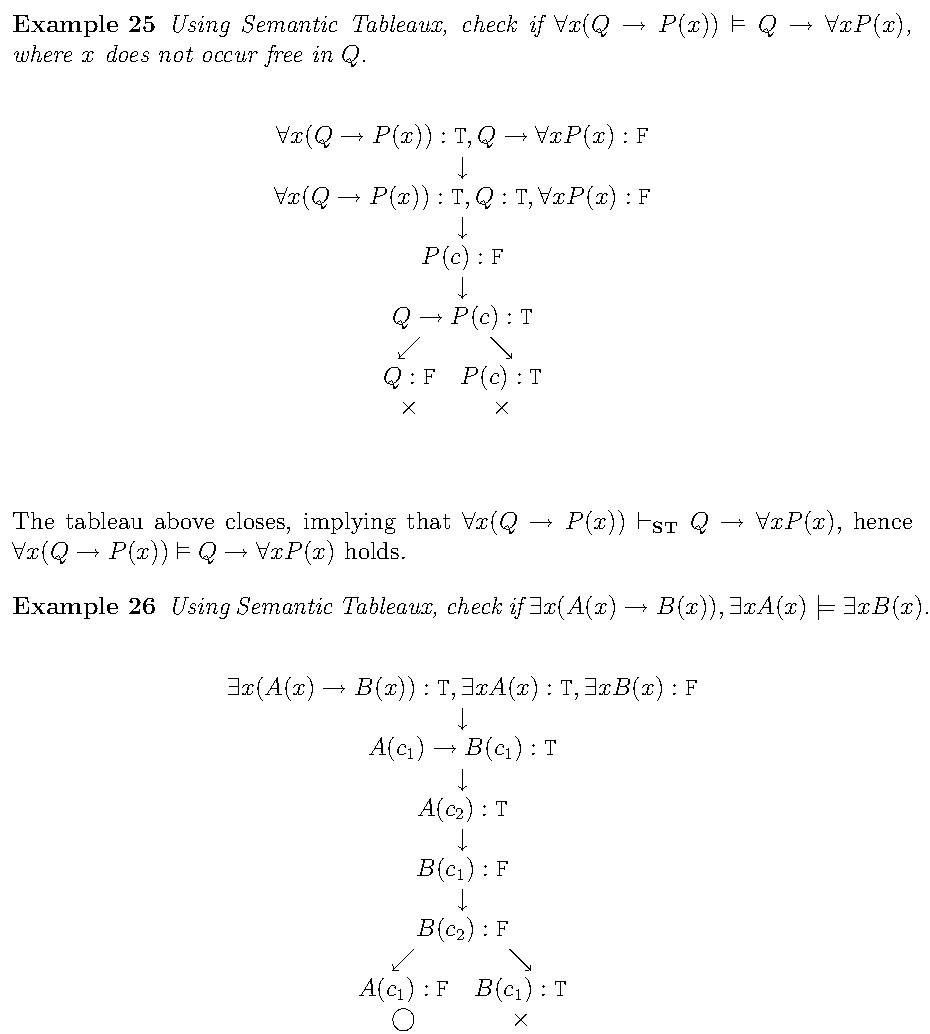
\includegraphics[scale=0.6]{./figures/tableaux.pdf}
\end{figure}